\section{Code Explanation}
\lstset{
    language=Python,
    basicstyle=\color{blue}
}

\section*{\textcolor{red}{Crop Recommendation System}}
%\vspace{4\baselineskip}
\subsection{Importing Necessary Libraries:}
\begin{lstlisting}[language=Python]
import pandas as pd
import matplotlib.pyplot as plt
import sklearn
from sklearn.model_selection import train_test_split
from sklearn.neighbors import KNeighborsClassifier
from sklearn.metrics import confusion_matrix
from sklearn.metrics import accuracy_score
from sklearn.svm import SVC
import seaborn as sns


\end{lstlisting}
%\vspace{7\baselineskip}

\subsection{Data Understanding:}
\begin{lstlisting}[language=Python]
    df=pd.read_csv("cropdata.csv")
    df
\end{lstlisting}

\begin{figure}[ht]
    \centering
    \caption{Loading the dataset}
    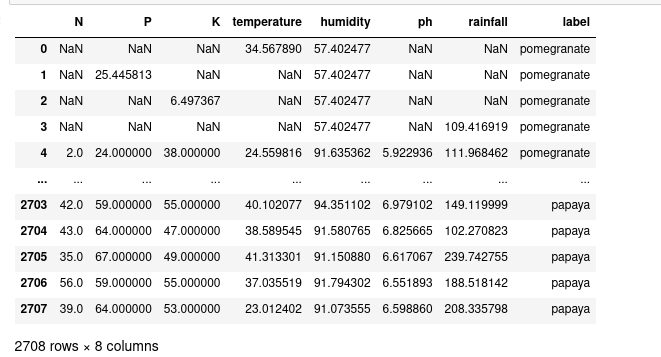
\includegraphics[width=7in,height=3in]{data.jpg}
    
    \label{fig:data}
\end{figure}
\vspace{2\baselineskip}
\begin{lstlisting}[language=Python]
    df.info()
\end{lstlisting}
\begin{figure}[ht]
    \centering
    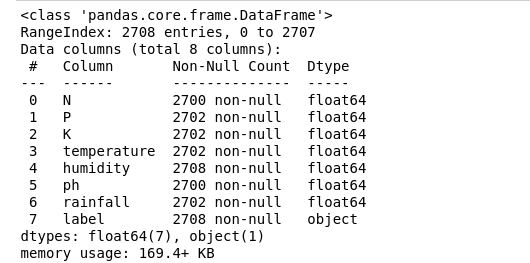
\includegraphics[width=5in,height=3in]{info.png}
    \caption{Data info}
    \label{fig:data}
\end{figure}


\hspace{2in}\textcolor{violet}{dtype: float64(7), object(1))}
\newline
\textcolor{gray}{\hspace{0.5cm}Dataframe contained 8 null values and the label is object}
%\hspace{2in}\textcolor{green}{dtype: float64(7), object(1))}
\begin{lstlisting}[language=Python]
    df.corr()
\end{lstlisting}
\begin{figure}[ht]
    \centering
    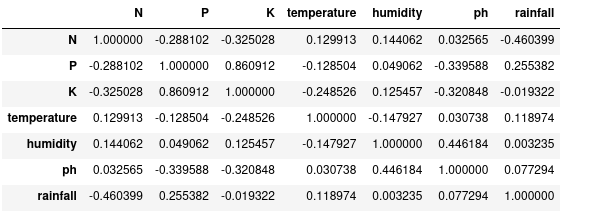
\includegraphics[width=7in,height=3in]{corr.png}
    \label{fig:data}
\end{figure}

\textcolor{gray}{\hspace{0.5cm}It calculates the relationship between each column.}
\newline
\begin{lstlisting}[language=Python]
df.shape()
\end{lstlisting}
\hspace{2in}\textcolor{red}{Output:}
\newline
\hspace{2in}\textcolor{violet}{(2708, 8)}
\newline
\textcolor{gray}{\hspace{0.5cm}The dataset contains 2708 rows and 8 columns}
\newline
\begin{lstlisting}[language=Python]
df.describe()
\end{lstlisting}
\newline
\textcolor{gray}{\hspace{0.5cm}It returns the description of the data in the dataframe}
\begin{figure}[ht]
    \centering
    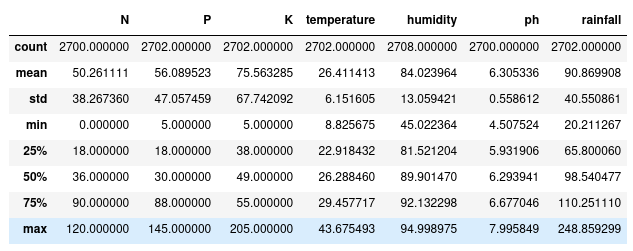
\includegraphics[width=5in,height=3in]{describe.png}
    \label{fig:data}
\end{figure}

\vspace{3\baselineskip}
 \begin{lstlisting}[language=Python]
df.head()
\end{lstlisting}
\newline
\textcolor{gray}{\hspace{0.5cm}It returns first five values}
\begin{figure}[ht]
    \centering
    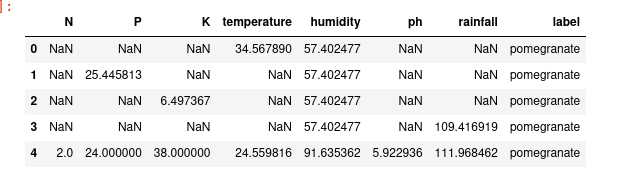
\includegraphics[width=4in,height=2in]{head.png}
    \label{fig:data}
\end{figure}
 
\subsection{Data Preprocessing:}
\begin{lstlisting}[language=Python]
    df.duplicated()
\end{lstlisting}
\newline
\textcolor{red}{\hspace{0.5cm}Checking of duplicate values}
\begin{figure}[ht]
    \centering
    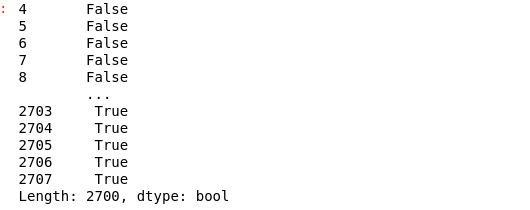
\includegraphics[width=5in,height=2in]{duplicates.png}
    \label{fig:data}
\end{figure}

\textcolor{gray}{\hspace{0.5cm}It shows that our dataset contain some duplicate values.Next process is to replace the null values}

%\vspace{5\baselineskip}
\textcolor{red}{Replacing the null values}
\begin{lstlisting}[language=Python]
x=df["N"].mean()
df["N"].fillna(x,inplace=True)
x=df["P"].mean()
df["P"].fillna(x,inplace=True)
x=df["K"].mean()
df["K"].fillna(x,inplace=True)
x=df["temperature"].mean()
df["temperature"].fillna(x,inplace=True)
x=df["humidity"].mean()
df["humidity"].fillna(x,inplace=True)
x=df["ph"].mean()
df["ph"].fillna(x,inplace=True)
x=df["rainfall"].mean()
df["rainfall"].fillna(x,inplace=True)
print(df.to_string())
\end{lstlisting}

\begin{figure}[ht]
    \centering
    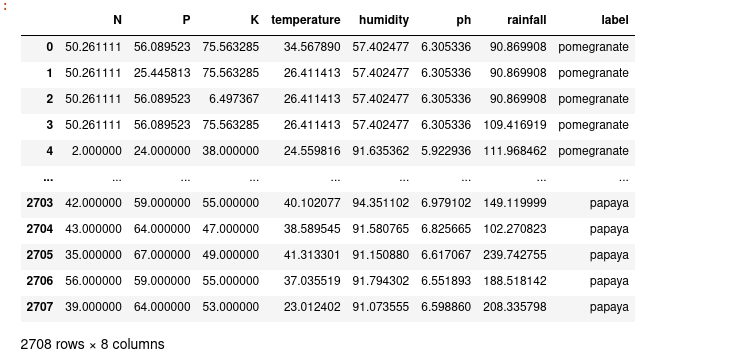
\includegraphics[width=7in]{replace.png}
\end{figure}

\textcolor{gray}{\hspace{0.5cm}It indicates that the null values are replaced by mean value of the entire column of each parameter in the dataset.}

\hspace{2in}\textcolor{blue}{df.info()}

\begin{figure}[ht]
    \centering
    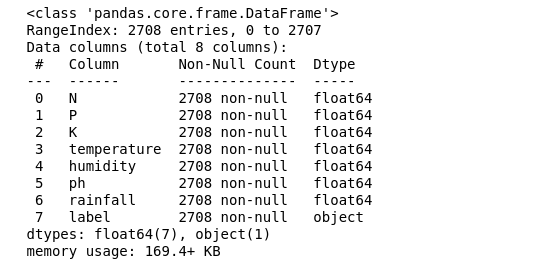
\includegraphics[width=4in,height=1.2in]{info1.png}
\end{figure}


\begin{lstlisting}[language=Python]
  x=df["label"].nunique()
  print("No.of crops:",x)  
\end{lstlisting}
\hspace{2in}\textcolor{red}{Output:}
\newline
\hspace{2in}\textcolor{violet}{No.of crops: 9}

\textcolor{grey}{\hspace{0.5cm}It represents the no.of crops  present in the dataset.}
%\vspace{7\baselineskip}

\begin{lstlisting}[language=Python]
    df=df.rename(columns={"label":"crop"})
    df
\end{lstlisting}

\begin{figure}[ht]
    \centering
    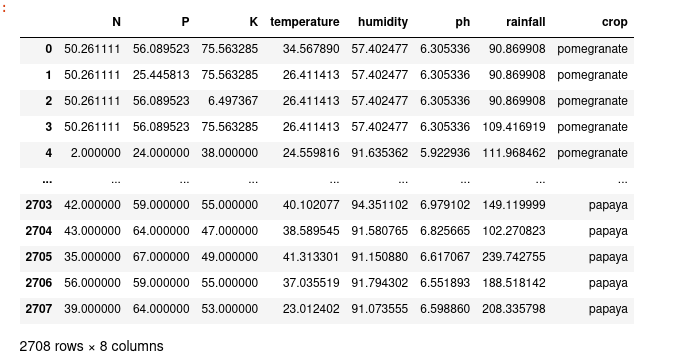
\includegraphics[width=7in]{rename.png}
\end{figure}
\textcolor{grey}{\hspace{0.5cm}From the above, the column name changes from label to crop}
\newline
\begin{lstlisting}[language=Python]
print("Crop names:")
for crop in df["label"].unique():
    print(crop)
\end{lstlisting}
\begin{figure}[ht]
    \centering
    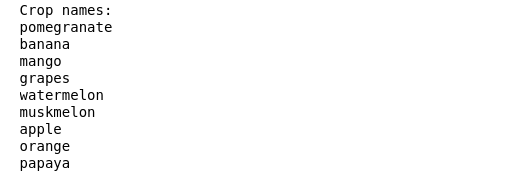
\includegraphics[width=4in]{crop.png}
\end{figure}
\vspace{5\baselineskip}
\textcolor{grey}{\hspace{0.5cm}We can print the particular crop data.}

\begin{lstlisting}[language=Python]
    crop_name="papaya"
    filtered_df=df[df["crop"]==crop_name]
    filtered_df
\end{lstlisting}

\begin{figure}[ht]
    \centering
    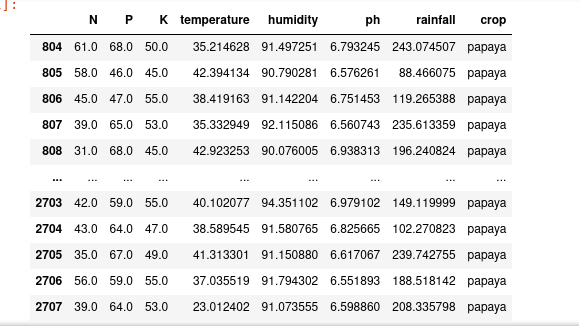
\includegraphics[width=5in]{particular.png}
\end{figure}
\subsection*{Evolution measures}

\textcolor{green}{\hspace{0.5cm}{Using Support Vector Machine(SVM) Algorithm:}}
\begin{lstlisting}[language=Python]
  X = data.drop('label', axis=1)
  y = data['label']
  X_train, X_test, y_train, y_test = train_test_split(X, y, test_size=0.3, 
  random_state=42)
  svm = SVC()
  svm.fit(X_train, y_train)
\end{lstlisting}
\begin{lstlisting}[language=Python]
cm = confusion_matrix(y_test, y_pred)
plt.figure(figsize=(8, 6))
sns.heatmap(cm, annot=True, cmap="Blues", fmt="d", xticklabels=
svm.classes_ ,yticklabels=svm.classes_)
plt.xlabel("Predicted Labels")
plt.ylabel("True Labels")
plt.title("Confusion Matrix")
plt.show()
\end{lstlisting}

\begin{figure}[h]
\centering
 \footnotesize
 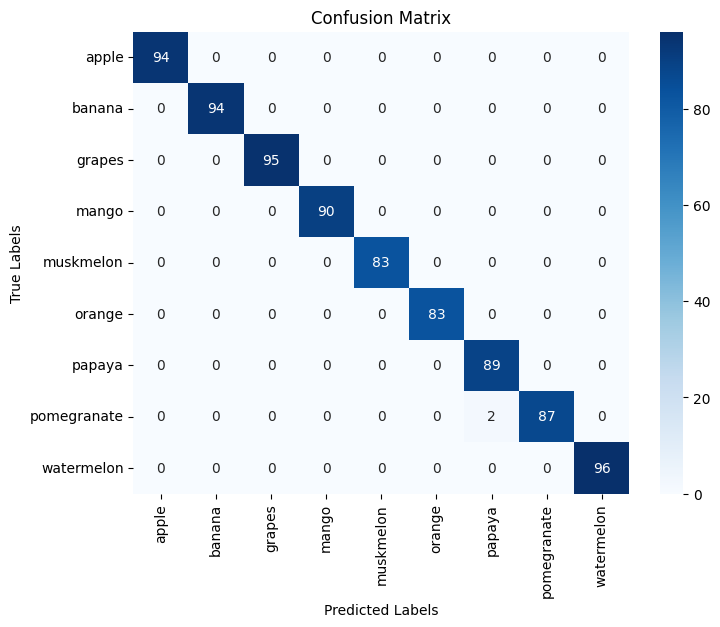
\includegraphics[width=3in,height=2in]{confusion.png}
\label{fig:dunnhalftone}
\end{figure}

\begin{lstlisting}[language=Python]
  y_pred = svm.predict(X_test)
  accuracy = accuracy_score(y_test, y_pred)
  print("Accuracy:", accuracy)
\end{lstlisting}
\hspace{2in}\textcolor{red}{Output:}
\newline
\hspace{2in}\textcolor{grey}{Accuracy: 0.997539975399754}

%\vspace{2\baselineskip}
\textcolor{green}{\hspace{0.5cm}{Using K-Nearest Neighbour(KNN)  Algorithm:}}
\begin{lstlisting}[language=Python]
  X = data.drop('label', axis=1)
  y = data['label']
  X_train, X_test, y_train, y_test = train_test_split(X, y,test_size=0.3, 
  random_state=42)
  k = 19 
  knn = KNeighborsClassifier(n_neighbors=k)
  knn.fit(X_train, y_train)
\end{lstlisting}
\begin{lstlisting}[language=Python]
cm = confusion_matrix(y_test, y_pred)
plt.figure(figsize=(8, 6))
sns.heatmap(cm, annot=True, cmap="Blues", fmt="d", xticklabels=
knn.classes_,yticklabels=knn.classes_)
plt.xlabel("Predicted Labels")
plt.ylabel("True Labels")
plt.title("Confusion Matrix")
plt.show()
\end{lstlisting}

\begin{figure}[h]
\centering
 \footnotesize
 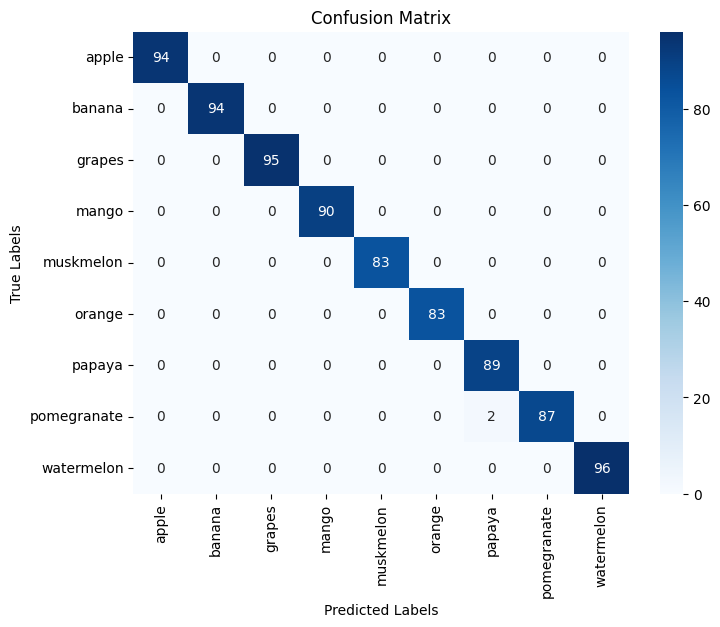
\includegraphics[width=3in,height=2in]{confusion.png}
\label{fig:dunnhalftone}
\end{figure}

\begin{lstlisting}[language=Python]
  y_pred = knn.predict(X_test)
  accuracy = accuracy_score(y_test, y_pred)
  print("Accuracy:", accuracy)
\end{lstlisting}

\hspace{2in}\textcolor{red}{Output:}
\newline
\hspace{2in}\textcolor{grey}{Accuracy: 0.997539975399754}
\subsection*{Predictions by the model}
\textcolor{green}{\hspace{0.5cm}{Using KNN  Algorithm:}}
\begin{lstlisting}[language=Python]
  new_data = {
    'N': 50,  
    'P': 30,  
    'K': 20, 
    'temperature': 28,  
    'humidity': 70,  
    'ph': 6.5,  
    'rainfall': 100  
  }
  new_input = pd.DataFrame(new_data, index=[0])
  predicted_label = knn.predict(new_input)
  print("Predicted label:", predicted_label[0])
\end{lstlisting}
 
\hspace{2in}\textcolor{red}{Output:}
\newline
\hspace{2in}\textcolor{grey}{Predicted label: mango}
\newline
\textcolor{green}{\hspace{0.5cm}{Using SVM Algorithm:}}
\begin{lstlisting}[language=Python]
  new_data = {
    'N': 50,  
    'P': 30,  
    'K': 20, 
    'temperature': 28,  
    'humidity': 70,  
    'ph': 6.5,  
    'rainfall': 100  
  }
  new_input = pd.DataFrame(new_data, index=[0])
  predicted_label = svm.predict(new_input)
  print("Predicted label:", predicted_label[0])

\end{lstlisting}
\hspace{2in}\textcolor{red}{Output:}
\newline
\hspace{2in}\textcolor{grey}{Predicted label: mango}